% tikz source used to create the sellar tree hierarchy diagram in the sellar tutorial

\documentclass[tikz, border=5pt]{standalone}
\usepackage{tikz}
%
\usetikzlibrary{trees}
\begin{document}
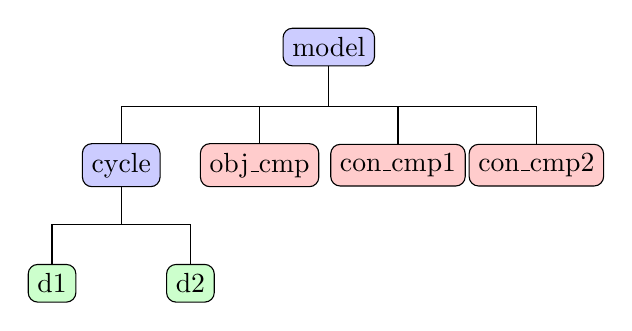
\begin{tikzpicture}[
  group/.style={rectangle,draw,fill=blue!20, rounded corners=.8ex},
  component/.style={rectangle,draw,fill=green!20,rounded corners=.8ex},
  exec_comp/.style={rectangle,draw,fill=red!20,rounded corners=.8ex},
  first/.style={level distance=6ex},
  second/.style={level distance=12ex},
  third/.style={level distance=18ex},
  level 1/.style={sibling distance=5em}]
    % Parents
    \coordinate
      node[group]{model}
    [edge from parent fork down]
    % Children and grandchildren
    child{node[group]{cycle}
      child{node[component]{d1}}
      child{node[component]{d2}}}
    child{node[exec_comp]{obj\_cmp}}
    child{node[exec_comp]{con\_cmp1}}
    child{node[exec_comp]{con\_cmp2}};
\end{tikzpicture}
\end{document}